\section{Auswahl der Algorithmen}

Es gibt vier unterschiedlichen Algorithmen auszuwählen.
\begin{enumerate}
	\item Linear Least Square
	\item Least Median Square 
	\item Residual Weighting Algorithm
	\item Non-Linear Least Square
\end{enumerate} 

In dieser Projektarbeit werden Linear Least Square und Least Median Square verwendet. Mittels Linear Least Square kann die gesuchte Position gerechnet werden, aber die Tatsache ist es, dass die fehlerbehaftete Distanzmessungen wegen Non Line of Sight (NLOS)-Verbindung immer vorhanden sind. Deswegen haben berechnete Ergebnisse keine Genauigkeit. Um die optimierte Position zu finden, muss die fehlerbehaftete Distanzmessungen gefiltert werden. Dafür spielt Medien Least Square wichtige Rolle.

Um die beide Algorithmen besser zu verstehen, wird die Lokalisierung eines Sensors unter mathematischen Aspekten betrachtet. Im dreidimensionalen Raum befinden sich N Referenzpunkte (bekannte Sensoren) und ein gesuchter Punkt (unbekannter Sensor). P\textsubscript{1} bis P\textsubscript{N} sind die Referenzpunkte mit den Koordinaten (X\textsubscript{1}, Y\textsubscript{1}, Z\textsubscript{1}) bis (X\textsubscript{N}, Y\textsubscript{N}, Z\textsubscript{N}). P\textsubscript{lat} ist der gesuchte Punkt (X, Y, Z) und R\textsubscript{i} ist die gemessene Distanz von P\textsubscript{lat} zum Referenzpunkt P\textsubscript{i}. In mathematischen Aspekt ist P\textsubscript{lat} tatsächlich ein Schnittpunkt, in dem sich verschiedene Kugeln mit unterschiedlichen Radien im dreidimensionalen Raum überschneiden (vgl. Abb.1). 

\begin{figure}[H]
	\centering
	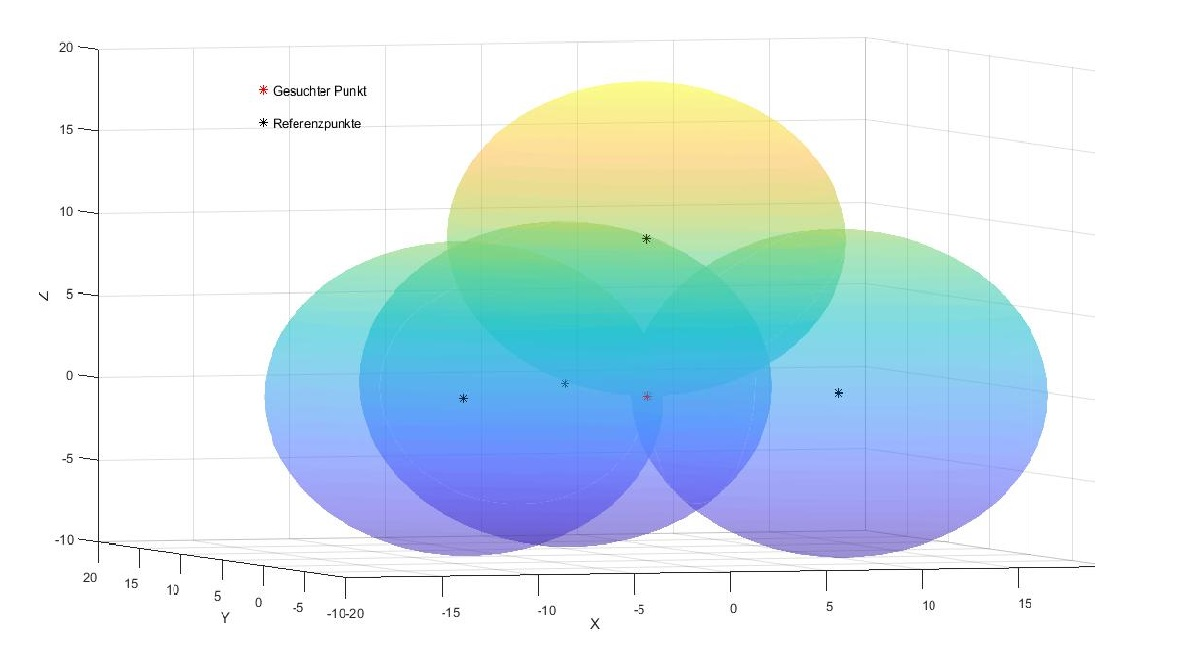
\includegraphics[scale=0.36]{img/Schnittpunkt_3D.jpg}
	\caption{Schnittpunkt verschiedenen Kugeln in einer 3D-Umgebung}
\end{figure}

